%! Suppress = MissingImport
%! Suppress = TooLargeSection
%! Suppress = SentenceEndWithCapital
%! Suppress = LineBreak
%! Suppress = MissingLabel
%! Suppress = Unicode

\documentclass[main.tex]{subfiles}

\begin{document}

    \section{Metody dowodzenia poprawności pętli.}

    \begin{itemize}
        \item \textbf{Asercja} - warunek logiczny wyrażający zależności między zmiennymi
        algorytmu w kontekście ich aktualnego stanu.
        \item \textbf{Asercja początkowa} - asercja określająca warunek wejściowy (warunek danych wejściowych) algorytmu.
        \item \textbf{Asercja końcowa} - asercja określająca wyniki algorytmu (warunek
        danych wyjściowych).
        \item Asercje początkowa i końcowa są znane w momencie definiowania
        problemu i poszukiwania algorytmu, stanowiąc \textbf{specyfikację algorytmu}
    \end{itemize}

    \begin{itemize}
        \item Algorytm A ma własność \textbf{określoności obliczeń} względem warunku $\alpha$, jeśli dla każdych danych spełniających warunek $\alpha$ działanie algorytmu A nie zostanie zerwane
        (oznaczenie $obl ( \alpha, A )$ ).
        \item Algorytm A ma \textbf{własność stopu} względem warunku $\alpha$, jeśli dla każdych danych spełniających warunek $\alpha$ działanie algorytmu A nie ciągnie się w nieskończoność (oznaczenie stop $( \alpha, A )$ ).
        \item Algorytm A jest \textbf{częściowo poprawny} względem warunku początkowego $\alpha$ oraz warunku końcowego $\beta$, gdy dla każdych danych spełniających warunek początkowy $\alpha$, jeżeli działanie algorytmu A dochodzi do końca, wyniki spełniają warunek końcowy $\beta$ (oznaczenie cp $( \alpha, A, \beta)$ ).\\
        $cp ( \alpha, z \leftarrow w, \beta ) \iff ( \alpha \Rightarrow \beta|_{z \leftarrow w})$\\
        Przy asercji początkowej $\alpha$ i asercji końcowej $\beta$ podstawienie z $\leftarrow$ w jest częściowo poprawne wtedy i tylko wtedy, gdy
        poprawna jest implikacja od asercji $\alpha$ do asercji $\beta$, z zastąpieniem każdego wystąpienia zmiennej z podstawianym
        wyrażeniem w.
        \item Algorytm A jest \textbf{całkowicie poprawny} (semantycznie poprawny) względem warunku
        początkowego $\alpha$ oraz warunku końcowego $\beta$, jeśli ma własność określoności obliczeń
        względem warunku $\alpha$, ma własność stopu względem warunku $\alpha$ oraz jest częściowo
        poprawny względem warunku $\alpha$ i warunku $\beta$ (oznaczenie sp $( \alpha, A, \beta )$ ).
        \item Formalnie:
        $sp ( \alpha, A, \beta ) \iff obl ( \alpha, A ) \wedge stop ( \alpha, A ) \wedge cp ( \alpha, A, \beta )$
    \end{itemize}

    \newpage
    \section{Odwrotna Notacja Polska: definicja, własności, zalety i wady, algorytmy.}

    \begin{itemize}
        \item notacja postfiksowa,
        \item jednoznacznie wyznacza kolejność wykonywania działań,
        \item pozwala na całkowitą rezygnację z nawiasów.
        \item Zalety:
        \begin{itemize}
            \item ułatwione obliczenia na komputerze - wykorzystuje jedynie stos
            \item prosty algorytm konwersji między standardowym zapisem infiksowym a ONP
            wykorzystywany w wielu algorytmach wykorzystujących jako wejście zapis działań
            brak konieczności stosowania nawiasów
        \end{itemize}
        \item Wady:
        \begin{itemize}
            \item mniej czytelny dla człowieka (wymaga przyzwyczajenia)
            \item podczas zapisu na kartce ``12 34'' + może wyglądać jak ``123 4'' + (xD)
        \end{itemize}
    \end{itemize}

    \subsection{Algorytm obliczenia wartości wyrażenia ONP}
    \begin{verbatim}
        Dla wszystkich symboli z wyrażenia ONP wykonuj:
        jeśli i-ty symbol jest liczbą, to odłóż go na stos,
        jeśli i-ty symbol jest operatorem (funkcją):
        zdejmij ze stosu oczekiwaną liczbę elementów  (parametrów)
        odłóż na stos wynik działania operatora (wynik funkcji)
        Zdejmij ze stosu wynik.
    \end{verbatim}

    \subsection{Algorytm konwersji z notacji infiksowej do ONP}

    \begin{verbatim}
        do {
        weź_kolejny_element_z_wejścia;
        if ( element_jest_operandem )
        dopisz_element_na_wyjscie;
        else // element jest operatorem, przecinkiem lub nawiasem
        if ( element_jest_operatorem o1) {
        while ( (lewa łączność(o1) and
        prior_(operatora_na_stosie o2) >= prior_(elementu o1))
        or (prawa łączność(o1) and
        prior_(operatora_na_stosie o2) > prior_(elementu o1)) ){
        przepisz_operator_(o2) ze_stosu_na_wyjscie ;
        }
        wstaw_operator_(o1) _na_wyjscie ;
        }
        else
        if ( element == '(' )
        wstaw_element_na_stos;
        else
        if ( element jest ',')
        zignoruj go i wczytaj kolejny symbol z wejścia
        else
        if( element == ')' ) {
        while( na_stosie_jest element różny od '(' )
        przepisz_go_na_wyjscie;
        Usuń_ze_stosu_( ;
        }
        } while(!koniec_danych);
        while( niepusty_stos )
        przepisz_element_ze_stosu_na_wyjscie;
    \end{verbatim}

    \newpage

    \section{Modele obliczeń: maszyna Turinga.}

    \begin{definition}
        \textbf{Formalna definicja maszyny Turinga}. Maszynę Turinga opisujemy poprzez krotkę:
        \[MT ~ = ~<Q, \Sigma, \delta, \tau, q_0, B, F >\]
        gdzie:
        \begin{itemize}
            \item $Q$ - skończony zbiór stanów,
            \item $q_0 \in Q$ - stan początkowy,
            \item $F \subset Q$ - zbiór stanów końcowych,
            \item $\tau$  - skończony zbiór dopuszczalnych symboli,
            \item $b \in \tau$  - symbol pusty,
            \item $\Sigma \subset \tau \ \{b\} $ - zbiór symboli wiejściowych,
            \item $\delta$ - funkcja sterująca.
            \begin{itemize}
                \item W wersji niedeterministycznej postaci maszyny Turinga:
                \[ \delta \subset (Q \times \tau)  \times (\tau \times \{\leftarrow, \rightarrow, \downarrow\}  \times Q)\]
                \item W wersji deterministycznej:
                \[ \delta : Q \times \tau \mapsto \tau \times \{\leftarrow, \rightarrow, \downarrow\} \times Q\]
            \end{itemize}
        \end{itemize}
    \end{definition}

    \begin{definition}
        \textbf{Tablica sterująca}. Dwuwymiarowa tablica indeksowana:
        \begin{itemize}
            \item Stanami w jednym wymiarze,
            \item Symbolami taśmy w drugim wymiarze.
        \end{itemize}
        Elementy tablicy
        \begin{itemize}
            \item Odpowiadają wszystkim parom stanu i czytanego symbolu stanowiąc dziedzinę
            funkcji sterowania $\delta$,
            \item Zawierają trójki działania maszyny, czyli wartości funkcji sterowania $\delta$.
        \end{itemize}
    \end{definition}

    \newpage

    \section{Modele obliczen: automat skończony, automat ze stosem.}
    \subsection{Automat skończony deterministyczny}
    \begin{definition}
        Automat skończony deterministyczny oznaczamy piątką parametrów: $\mathcal{A}$ = (S, A, f, $s_{0}$, T) gdzie: \\
        S - skończony zbiór stanów \\
        A - skończony alfabet wejściowy \\
        f - funkcja przejścia S$\times$A $\rightarrow$ S \\
        $s_{0}$ - stan początkowy $\in$ S\\
        T - zbiór terminali (stanów akceptujących) $\in$ S
    \end{definition}

    \begin{definition}
        Automaty $\mathcal{A}_{1}$ i  $\mathcal{A}_{2}$ są równoważne, jeżeli rozpoznają ten sam język, czyli: \\
        L($\mathcal{A}_{1}$) = L($\mathcal{A}_{2}$)
    \end{definition}

    \begin{definition}
        Każdy automat $\mathcal{A}$ = (S, A, f, $s_{0}$, T) wyznacza w wolnym monoidzie $A^{*}$ prawą kongruencję automatową okresloną w następujący sposób: \\
        $\forall$u,v $\in A^{*}$ \\
        $u \sim_\mathcal{A}$ v $\Leftrightarrow f(s_{0}, u) = f(s_{0}, v)$
    \end{definition}

    \begin{definition}
        Niech $L \subset  A^{*}$ będzie dowolnym językiem, a $u \in A^{*}$ dowolnym słowem.
        Pochodną Brzozowskiego (residuum) z języka L względem słowa u nazywamy język \\
        $u^{-1}L = \{w \in A^{*}$  :  $uw \in L \}$
    \end{definition}

    \begin{definition}
        Automat ilorazowy to automat, w którym stanami są klasy równoważności
    \end{definition}

    \begin{definition}
        Monoidem przejśc automatu $\mathcal{A}$ nazywamy monoid \\
        $\mathcal{M(A)}$ = $\tau_\mathcal{A}(A^*) \subset S^{S}$
    \end{definition}

    \begin{definition}
        Każdy język skończony jest akceptowany przez pewien deterministyczny automat skończony
    \end{definition}

    \subsection{Automat skończony niedeterministyczny}
    \begin{definition}
        Automat skończony niedeterministyczny oznaczamy piątką parametrów: $\mathcal{A_{ND}}$ = (S, A, f, $S_{0}$, T) gdzie: \\
        S - skończony zbiór stanów \\
        A - skończony alfabet wejściowy \\
        f - funkcja przejścia S$\times$A $\rightarrow$ $\mathcal{P}$(S) \\
        $S_{0}$ - zbiór stanów początkowych $\subset$ S\\
        T - zbiór terminali (stanów akceptujących) $\in$ S \\

        Słowo x jest akceptowane gdy $f^{*}$($S_{0}$, x) $\cap$ T $\neq \emptyset$
    \end{definition}

    \subsection{Automat ze stosem}
    \begin{definition}
        Automat ze stosem to $\mathcal{AS}$ = (A, $A_{S}$, Q, f, $s_{0}$, $z_{0}$, $Q_{F}$) gdzie: \\
        A - jest alfabetem \\
        $A_{S}$ - jest dowolnym, skończonym i niepustym zbiorem zwanym alfabetem stosu \\
        Q - jest dowolnym, skończonym i niepustym zbiorem zwanym zbiorem stanów \\
        f: $A_{s} \times Q \times (A \cup \{1\}) \rightarrow \mathcal{P}_{sk}(A^{*}_{S} \times Q)$ jest funkcją przejść \\
        $q_{0} \in Q$ jest stanem początkowym \\
        $z_{0} \in A_{S}$ jest symbolem początkowym stosu \\
        $Q_{F} \subset Q$ zbiorem stanów końcowych
    \end{definition}

    \newpage

    \section{Złożoność obliczeniowa - definicja notacji: $O, \Omega, \Theta$.}
    \begin{definition}
        Niech$f, g, h: \mathbb{N} \rightarrow \mathbb{R}_{+} \cup \{0\}$, wtedy:
        \begin{itemize}
            \item $\mathbf{f(n) = O(g(n))}$ - f jest \textbf{co najwyżej rzędu} g, gdy istnieje $c > 0$ i
            $n_0 \in \mathbb{N}$, takie że $f(n)  \leq cg(n)$ dla każdego $n \geq n_0$.
            \item $\mathbf{f(n) = \Omega(g(n))}$ - f jest \textbf{co najmniej rzędu} g, gdy $g(n) = O(f(n))$
            \item $\mathbf{f(n) = \Theta(g(n))}$ - f jest \textbf{dokładnie rzędu} g, gdy $f(n) = O(g(n))$
            i $f(n) = \Omega(g(n))$.
        \end{itemize}
    \end{definition}

    \newpage

    \section{Złożoność obliczeniowa - pesymistyczna i średnia.}

    \begin{definition}
        Niech:
        \begin{itemize}
            \item $D_n$ - zbiór danych rozmiaru n,
            \item $t(d)$ - liczba operacji dominujących,
            \item $X_n$ - zmienna losowa dla $t(d) \in D_n$,
            \item $p_{kn}$ - rozkład prawdopodbieńdstwa zmiennej $X_n$.
        \end{itemize}

        \textbf{Optymistyczna złożoność czasowa}:
        \begin{align*}
            Opt(n) = inf\{t(d) : d \in D_n\}
        \end{align*}

        \textbf{Średnia złożoność czasowa}:
        \begin{align*}
            A(n) = ave(X_n) = \sum_{k \geq 0}kp_{nk}
        \end{align*}

        \textbf{Pesymistyczna złożoność czasowa}:
        \begin{align*}
            W(n) = sup\{t(d) : d \in D_n\}
        \end{align*}
    \end{definition}

    \begin{definition}
        \textbf{Koszt amortyzowany}

        Koszt amortyzowany operacji jest średnim czasem wykonania przypadającym na jedną operację w pesymistycznym ciągu operacji. Koszt amortyzowany różni się od kosztu średniego tym, że bierze pod uwagę pesymistyczny ciąg operacji i nie jest metodą probabilistyczną.

    \end{definition}

    \textbf{Przykład:}

    Tablica dynamiczna (np. vector w C++) podwaja swoją długość w przypadku, gdy jest pełna i dodajemy do niej nowy element.
    Alokuje wówczas dwukrotnie większą pamięć i kopiuje wszystkie elementy.
    Koszt takiego rozszerzenia jest równy $\theta(n)$.\\

    Obliczmy koszt amortyzowany wstawienia elementu do tablicy przy wstawieniu $n$ elementów ($n = 2^k,\; k \in \mathbb{N}$),
    zaczynając od pustej tablicy o długości 1.

    \[T(n) = \frac{1}{n} \left(1 + 2 + 4 + \cdots + \frac{n}{2}\right) =
    \frac{1}{n} \sum_{i = 0}^{log_2(n) - 1}2^i
    = \frac{n - 1}{n} = 1 - \frac{1}{n} = \theta(1)\]

    Zatem sumaryczny koszt wstawienia do takiej tablicy n elementów jest równy $\theta(n)$

    \newpage

    \section{Metoda "dziel i zwyciężaj": zalety i wady.}

    Algorytmy "dziel i zwyciężaj" podlegają poniższemu schematowi:

    \begin{enumerate}
        \item
        \textbf{Dziel}

        Dany problem dzielony jest rekurencyjnie na podproblemy, aż do uzyskania przypadków
        bazowych.

        \item
        \textbf{Zwyciężaj}

        Rozwiązujemy przypadki bazowe (najczęściej jest to możliwe w
        czasie stałym).

        \item
        \textbf{Łącz}

        Wyniki otrzymane z podproblemów są łączone aż do uzyskania wyniku danego problemu
    \end{enumerate}

    \subsection{Zalety}

    \begin{itemize}
        \item Algorytm podzielony jest na trzy ortogonalne części: dziel (\textit{divide}),
        zwyciężaj (\textit{conquer}) i łącz (\textit{merge / combine}), co ułatwia jego
        zrozumienie jak i analizę.

        \item Możliwość łatwego przekształcenia algorytmu w algorytm równoległy (przy pomocy
        wzorca redukcji / dekompozycji asynchronicznej).

        \item Optymalne użycie pamięci podręcznej (\textit{cache}): problemy dostatecznie małe
        (w szczególności bazowe) rozwiązywane są w pamięci
        nieprzekraczającej wielkości pamięci podręcznej.

        \item Znacząco lepsza złożoność obliczeniowa od bardziej prymitywnych
        podejść (jak na przykład \textit{brute-force}).
    \end{itemize}

    \subsection{Wady}

    \begin{itemize}
        \item W przypadku podziału na dwa i więcej podproblemy uzyskujemy rekurencję nieliniową.
        Oznacza to, że przekształcenie algorytmu rekurencyjnego w algorytm iteracyjny
        jest nietrywialne (w szczególności nie zostanie to wykonane przez
        kompilator).


        \item Potencjalnie wysoka złożoność pamięciowa algorytmu rekurencyjnego / iteracyjnego ze stosem.
        Ponadto rozmiar stosu może przekroczyć pamięć komputera.


        \item Możliwość wielokrotnego rozwiązywania identycznych problemów.

        Problem ten rozwiązuje się stosując praktyki należące do programowania dynamicznego
        (np. \textit{memoization}).

    \end{itemize}

    \subsection{Przykłady}

    \begin{itemize}
        \item Binsearch
        \item Merge sort
        \item Quicksort
        \item Szybkie potęgowanie
        \item Algorytm Karacuby (szybkie mnożenie liczb całkowitych)
        \item Szybka transformata Fouriera
        \item Algorytm znajdowania otoczki wypukłej
    \end{itemize}


    \newpage

    \section{Lista: ujęcie abstrakcyjne, możliwe implementacje i ich złożoności.}
    \begin{definition}
        Lista jest abstrakcyjną strukturą danych (ADT), która posiada następujące właściwości
        \begin{itemize}
            \item Przechowuje elementy \textbf{tego samego typu}
            \item Wykorzystuje pamięć w sposób \textbf{dynamiczny lub statyczny}
            \item Dostęp do danych jest \textbf{sekwencyjny}
            \item Elementy w liście sa \textbf{liniowo uporządkowane} zgodnie z ich pozycją na liście
            \begin{itemize}
                \item element $a_i$ znajduje się na pozycji ‘i’
                \item element $a_i$ poprzedza $a_{i+1}$ dla i=$1,2,\cdots,n-1$
                \item element $a_i$ następuje po $a_{i-1}$ dla i=$2,\cdots,n$
            \end{itemize}
            \item Wyróżnia się dwa podstawowe sposoby implementacji listy jako ADT
            \begin{itemize}
                \item Tablica
                \item Lista wiązana
            \end{itemize}
        \end{itemize}
    \end{definition}

    \begin{definition}
        W sensie matematycznym lista jest skończonym ciągiem elementów ustalonego typu
        Node: $a_1, a_2, \cdots , a_n, , n \geq 0$
        przy czym Node, zwany typem bazowym, może być np. typem \textbf{klasy, struktury, int,
        string} itp.
    \end{definition}

    \subsection{Implementacja za pomocą tablic (array)}
    Tablica wykorzystuje pamięć w sposób \textbf{statyczny}. Oznacza to, że ma z góry określony rozmiar oraz pewna jej część może być niewykorzystana. Tablica posiada zmienne wskazujące na jej maksymalny rozmiar, ilość zajętych miejsc. Indeksowanie elementów zazwyczaj zaczyna się od 0 i kończy na maxsize-1.


    \subsection{Implementacja za pomocą Listy Wiązanej (Linked List)}
    Rozróznia się dwa podstawowe rodzaje:
    \begin{enumerate}
        \item Lista wiązana \textbf{jednokierunkowa} \\
        Z każdego elementu możliwe jest przejście do jego następnika NEXT
        \item Lista wiązana \textbf{dwukierunkowa} \\
        Z każdego elementu możliwe jest przejscie do jego następnika NEXT i poprzednika PREV
    \end{enumerate}

    W liście wiązanej wyróżnia się dwie podstawowe zmienne typu Node potrzebne do jej obsługi

    \begin{enumerate}
        \item HEAD
        \item TAIL
    \end{enumerate}

    Dodatkowo, lista wiązana jest \textbf{cykliczna} jeżeli

    \begin{enumerate}
        \item{$next(TAIL) \rightarrow HEAD$}
        \item{$prev(HEAD) \rightarrow TAIL$}
    \end{enumerate}

    Pojedynczy element listy jest klasą lub strukturą, zwyczajowo nazywa się Node (węzeł). Przechowuje pole data o pożądanym typie danych oraz wskaźnik (wskaźniki) na element następny (i poprzedni).
    \\
    Przykład implementacji struktury Node w C++

    \begin{verbatim}
        struct Node {
        int data;
        struct Node* next;
        struct Node* prev;
        };
    \end{verbatim}
    \newpage
    Przykład implementacji klasy Node w Java

    \begin{verbatim}
        class Node<E> {
        E data;
        Node<E> next;
        Node<E> prev;
        };
    \end{verbatim}

    Przykład implementacji klasy LinkedList w Java
    \begin{verbatim}
        class LinkedList<E> {
        Node<E> head; // head of the list
        Node<E> tail; // tail of the list
        int counter = 0;
        ...
        }
    \end{verbatim}

    Operacje i złożoności

    \begin{enumerate}
        \item
        \begin{verbatim}
            CREATE(l: List)
        \end{verbatim}
        Tworzy nową listę \\
        O(1) - czas stały
        \item
        \begin{verbatim}
            APPEND(l: List; d: Data)
        \end{verbatim}
        Dodaje na końcu listy l rekord d \\
        O(1) - czas stały
        \item
        \begin{verbatim}
            INSERT(l: List; d: Data; i: Integer)
        \end{verbatim}
        Dodaje rekord d do określonego miejsce i w liście l \\
        O(n) - czas liniowy
        \item
        \begin{verbatim}
            FIND(l: List; i: Integer)
        \end{verbatim}
        Znajduje i-ty w kolejności rekord z listy \\
        O(min(i, n)) - czas liniowy
        \item
        \begin{verbatim}
            DELETE(l: List; i: Integer)
        \end{verbatim}
        Usuwa -ity w kolejności rekord z listy \\
        O(min(i, n)) - czas liniowy
        \item
        \begin{verbatim}
            MAKENULL(l: List)
        \end{verbatim}
        Czyści listę, usuwając wszystkie rekordy \\
        O(1) - czas stały
    \end{enumerate}
    \newpage
    \section{Kolejka i kolejka priorytetowa: ujęcie abstrakcyjne, możliwe implementacje i ich złożoności.}
    \subsection{Kolejka}
    \begin{definition}
        Kolejka FIFO (First In First Out).

        Jest to lista, w której
        \begin{itemize}
            \item Wstawianie nowego elementu odbyca się na końcu kolejki \textbf{rear}
            \item Usuwanie elementu odbywa się na początku kolejki \textbf{front}\\
            \item Wyróżnia się dwa podstawowe sposoby implementacji kolejki
            \begin{itemize}
                \item Tablica cykliczna
                \item Lista wiązana
            \end{itemize}
        \end{itemize}
    \end{definition}

    Operacje i złożoności
    \begin{enumerate}
        \item
        \begin{verbatim}
            Create()
        \end{verbatim}
        Tworzy pustą kolejkę
        \item
        \begin{verbatim}
            isEmpty()
        \end{verbatim}
        Sprawdza czy kolejka pusta
        \item
        \begin{verbatim}
            Enqueue(x)
        \end{verbatim}
        Wstawia nowy element x
        \item
        \begin{verbatim}
            Front()
        \end{verbatim}
        Odczytuje pierwszy element w kolejce
        \item
        \begin{verbatim}
            Dequeue()
        \end{verbatim}
        Usuwa pierwszy element w kolejce i go zwraca
    \end{enumerate}

    \subsection{Sposoby implementacji kolejki}

    Na początku zauważmy, że \textbf{nieefektywną} realizacją kolejki w tablicy jest przyjęcie, że
    początek kolejki \textbf{front} będzie zawsze równy 0, a \textbf{rear} będzie indeksem do pierwszego
    wolnego elementu tablicy.\\


    Najbardziej \textbf{efektywnym} rozwiązaniem jest reprezentacja kolejki w \textbf{tablicy cyklicznej}.
    Operacje wstawiania i usuwania zwiększają pozycje końca i początku kolejki o 1 modulo
    rozmiar tablicy, wykorzystując metodę:
    \begin{verbatim}
        private int Add (int i){
        return (i+1) % maxSize; // reszta z dzielenia
        }
    \end{verbatim}

    \subsection{Kolejka Priorytetowa}
    \begin{definition}
        Kolejka Priorytetowa\\
        Jest to lista, w której
        \begin{itemize}
            \item Usuwany jest zawsze element o największej (najmniejszej) wartości
        \end{itemize}
    \end{definition}

    Operacje
    \begin{enumerate}
        \item
        \begin{verbatim}
            Insert(x, q)
        \end{verbatim}
        Wstawienie elementu ‘x’ do kolejki q
        \item
        \begin{verbatim}
            Max(Q)
        \end{verbatim}
        Odczyt największego elementu w kolejce (element ten jest zwracany jako wynik operacji, kolejka się nie zmienia)
        \item
        \begin{verbatim}
            Min(Q)
        \end{verbatim}
        Odczyt największego elementu w kolejce (element ten jest zwracany jako wynik operacji, kolejka się nie zmienia)
        \item
        \begin{verbatim}
            Delete_Max(Q)
        \end{verbatim}
        Usunięcie największego elementu z kolejki q
        \item
        \begin{verbatim}
            Delete_Min(Q)
        \end{verbatim}
        Usunięcie największego elementu z kolejki q
    \end{enumerate}


    \subsection{Sposoby implementacji kolejki priorytetowej}
    \begin{itemize}
        \item Lista - Tablica Nieuporządkowana
        NIEEFEKTYWNA!
        \item Lista - Tablica Uporządkowana Rosnąco (Malejąco)
        NIEEFEKTYWNA!
        \item Kopiec Max (Min)
    \end{itemize}

    \newpage

    \section{Algorytmy sortowania QuickSort i MergeSort: metody wyboru pivota w QS; złożoności.}

    \subsection{QuickSort.}

    \begin{minted}{python}
        def quickSort(arr, start, end):
        if (start < end)
        pivot = partition(arr, start, end)

        quickSort(arr, start, pivot - 1)
        quickSort(arr, pivot + 1, end)


        def partition (arr, start, end):
        pivot = arr[end]
        i = (start - 1)

        for j in range [start,end- 1]:
        if (arr[j] < pivot):
        i++;
        swap arr[i] and arr[j]

        swap arr[i + 1] and arr[end])
        return (i + 1)
    \end{minted}
    \textbf{Złożoność}: pesymistyczna - $O(n^2)$, średnia i optymistyczna - $O(nlog_2 n)$.\\

    \textbf{Sposoby wybrania pivota}
    \begin{enumerate}
        \item Pierwszy element
        \item Ostatni element
        \item Mediana z pierwszego, środkowego i ostatniego
        \item Losowy element
    \end{enumerate}
    \hfill \\\\

    \subsubsection{MergeSort.}

    \begin{minted}{python}
        def mergeSort (arr, start, end):
        if end > start:
        middle = (start+end)/2

        mergeSort (arr, start, middle)
        mergeSort (arr, middle+1, end)

        merge (arr, start, middle, right)
    \end{minted}
    \textbf{Złożoność:} pesymistyczna, średnia, optymistyczna - $O(nlogn)$.

    \newpage

    \section{Algorytm sortowania bez porównań (sortowanie przez zliczanie, sortowanie kubełkowe oraz sortowanie pozycyjne).}

    \subsection{CountSort.}
    \begin{minted}{python}
        def countSort (arr):
        count = []
        for a in arr:
        count[a] += 1

        i = 0;
        for j in range [0, arr.len]:
        while (count[i] == 0):
        i++
        arr[j] = i
        count[i]--
    \end{minted}
    \textbf{Złożoność:} $O(n+k)$.

    \subsection{BucketSort.}
    \begin{minted}{python}
        bucketSort (arr):
        n = arr.len
        buckets = [{} for i in range [1,n]]

        for a in arr:
        buckets[n*arr[i]].add(arr[i])

        for b in buckets:
        sort(b)

        i = 0
        for b in buckets:
        for a in b:
        arr[i++] = a
    \end{minted}
    \textbf{Złożoność:} pesymistyczna -  $O(n^2)$, średnia - $O\left(n + \frac{n^2}{k} + k\right)$.

    \subsection{RadixSort.}
    \begin{minted}{python}
        def radixSort (arr):
        for all digits ascending:
        countSort(arr, digit)
    \end{minted}
    \textbf{Złożoność:} $O(d(n+k))$, gdzie d jest liczbą cyfr.

    \newpage

    \section{Reprezentacja drzewa binarnego za pomocą porządków (preorder, inorder, postorder).}


    \begin{minted}{python}
        def preorder (v):
        func(v)
        preorder(v.left)
        preorder(v.right)

        def inorder (v):
        inorder(v.left)
        func(v)
        inorder(v.right)

        def postorder (v):
        postorder(v.left)
        postorder(v.right)
        func(v)
    \end{minted}

    Możemy odtworzyć wyjściowe drzewo, jeśli mamy inorder i post- lub pre-order.

    \newpage

    \section{Algorytmy wyszukiwania następnika i poprzednika w drzewach BST; usuwanie węzła.}

    \begin{definition}
        \textbf{Binarne drzewo poszukiwań (BST)} - dynamiczna struktura danych będąca drzewem binarnym, w którym lewe
        poddrzewo każdego węzła zawiera wyłącznie elementy o kluczach mniejszych niż klucz węzła a prawe poddrzewo
        zawiera wyłącznie elementy o kluczach nie mniejszych niż klucz węzła.
    \end{definition}

    \begin{verbatim}
        struct BSTNode {
        int key;
        struct BSTNode* parent;
        struct BSTNode* left;
        struct BSTNode* right;
        };
    \end{verbatim}

    \subsection{Wyszukiwanie następnika i poprzednika w BST.}
    \begin{definition}
        \textbf{Następnik} danego węzła to węzeł, który jest odwiedzany jako następny w przypadku przechodzenia drzewa
        metodą in-order. Sposób wyznaczenia nie wymaga porównywania żadnych kluczy, jest to w praktyce:
        \begin{itemize}
            \item skrajnie lewy element prawego poddrzewa węzła, jeśli posiada on prawe poddrzewo; wpp
            \item pierwszy napotkany przodek węzła, dla którego węzeł jest w lewym poddrzewie.
        \end{itemize}
    \end{definition}

    \begin{minted}{python}
        define BST_FIND_SUCCESSOR(Node):
        if (Node->right != NULL)
        return BST_SEARCH_MIN_KEY(Node->right)
        Node_tmp = Node->parent
        while (Node_tmp != NULL and Node_tmp->left != Node)
        Node = Node_tmp
        Node_tmp = Node_tmp->parent
        return Node_tmp
    \end{minted}


    \begin{definition}
        \textbf{Poprzednik} danego węzła to węzeł, który jest odwiedzany jako poprzedni w przypadku przechodzenia drzewa
        metodą in-order. Sposób wyznaczenia nie wymaga porównywania żadnych kluczy, jest to w praktyce:
        \begin{itemize}
            \item skrajnie prawy element lewego poddrzewa węzła, jeśli posiada on lewe poddrzewo; wpp
            \item pierwszy napotkany przodek węzła, dla którego węzeł jest w prawym poddrzewie.
        \end{itemize}
    \end{definition}

    \begin{minted}{python}
        define BST_FIND_PREDECESSOR(Node):
        if (Node->left != NULL)
        return BST_SEARCH_MAX_KEY(Node->left)
        Node_tmp = Node->parent
        while (Node_tmp != NULL and Node_tmp->right != Node)
        Node = Node_tmp
        Node_tmp = Node_tmp->parent
        return Node_tmp
    \end{minted}


    \subsection{Usuwanie węzła z BST.}

    \begin{theorem}
        Usuwanie węzła z BST wymaga rozważenia trzech przypadków:
        \begin{enumerate}
            \item w przypadku, gdy usuwany węzeł jest liściem wskaźnik do węzła w jego ojcu zastępowany jest wskaźnikiem do węzła pustego,
            \item w przypadku, gdy usuwany węzeł ma jednego syna to dany węzeł usuwamy a jego syna podstawiamy w miejsce usuniętego węzła,
            \item w przypadku, gdy usuwany węzeł ma dwóch synów to po jego usunięciu wstawiamy w jego miejsce węzeł, który jest jego następnikiem.
        \end{enumerate}
    \end{theorem}

    \newpage

    \section{B-drzewa: operacje i ich złożoność.}
    B-drzewa to rozszerzone drzewa BST.
    Jest ono typowo zoptymalizowane pod kątem operacji wejścia/wyjścia (np. odczytu z dysku twardego) - operacje długotrwałe takie jak odczyt węzła z dysku są wykonywane o wiele rzadziej niż dla typowych drzew BST, natomiast operacje takie jak wyszukanie odpowiedniej wartości w węźle załadowanym już do pamięci ram są praktycznie pomijane ze względu na nieporównywalnie większą szybkość ich wykonywania.
    B-drzewa mają ustalony rząd. \\
    \noindent B-drzewo rzędu K musi spełniać poniższe warunki:
    \begin{itemize}
        \item Korzeń jest liściem lub ma od 2 do K synów
        \item Wszystkie liście są na tym samym poziomie
        \item Każdy węzeł wewnętrzny (oprócz korzenia) ma od $\lceil K/2 \rceil$ do K synów. Jeżeli jakiś węzeł ma s synów, to musi mieć s-1 kluczy (wartości)
        \item Każdy liść zawiera od $\lceil K/2 \rceil - 1$ do K - 1 kluczy (wartości)
    \end{itemize}

    \noindent Warunek drugi gwarantuje niewielką wysokość drzewa (dla drzewa o n kluczach: w najgorszym wypadku $\log_{K/2} n/(K/2)$; w najlepszym wypadku $\log_{K} n/K$) \\

    \noindent Generalnie złożoność wszystkich operacji na B-drzewach wynosi $O(K \log_{K} n)$, gdzie n to ilość kluczy (wartości) w drzewie, a K to rząd drzewa.

    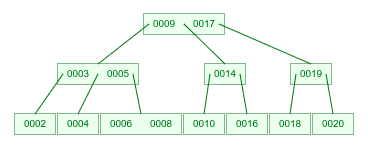
\includegraphics[]{b-trees/b-tree-example.png}

    \noindent Odmianą B-drzew są drzewa B+, które różnią się tym, że wszystkie wartości trzymane są w liściach oraz mają powiązania pomiędzy liśćmi (tak aby można było po kolei przejść wszystkie wartości w liściach).

    \subsection{Wyszukiwanie}
    Wyszukiwanie przebiega bardzo podobnie jak w drzewie BST, z tą różnicą, że nie mamy tylko lewego i prawego poddrzewa, a możemy mieć ich więcej, więc musimy zadecydować, do którego pójść.
    Oczywiście szukana wartość może również znajdować się na danym poziomie. Wtedy kończymy wyszukiwanie.
    Ponieważ rząd drzewa zazwyczaj jest wysoki (np. 1024), aby usprawnić wyszukiwanie zadanej wartości w danym węźle, najczęściej używamy wyszukiwania binarnego. \\

    \subsection{Wstawianie}
    Aby wstawić wartość wyszukujemy liść, do którego powinna trafić, a następnie wstawiamy ją w odpowiednie miejsce w tym liściu. \\
    \noindent Jeżeli jednak okazałoby się, że liść ma już za dużo kluczy (wartości) ($\geq K$), wtedy musimy go podzielić - jedną z wartości z liścia przenosimy w odpowiednie miejsce do rodzica, a jako prawego i lewego syna tej przeniesionej wartości wstawiamy odpowiednio liście powstałe po podzieleniu tego oryginalnego liścia. \\
    \noindent Jeżeli okazałoby się, że po przeniesieniu wartości z liścia do rodzica, rodzic ma za dużo kluczy (wartości), całą operację dzielenia powtarzamy rekurencyjnie na rodzicu - w razie potrzeby aż do korzenia. \\

    \subsection{Usuwanie}
    Usuwanie rozpoczynamy od znalezienia wartości, którą chcemy usunąć \\
    \noindent Następnie bierrzemy największą wartość z lewego podrzewa lub najmniejszą wartość z prawego poddrzewa i wstawiamy w miejsce usuwanego elementu \\
    \noindent Jeżeli w drzewie zostały naruszone warunki dotyczące ilości dozwolonych elementów w węźle, musimy to drzewo zrównoważyć. Proces ten jest generalnie dośc skomplikowany i ciężki do opisania algorytmem ze względu na mnogość możliwych przypadków, dlatego najlepiej spojrzeć na część praktyczną i przykłady.

    \newpage


    \section{Drzewa AVL: rotacje, operacje z wykorzystaniem rotacji i ich złożoność.}
    Drzewa AVL są odmianą drzew BST, w której dla każdego węzła mamy dodatkowy warunek: różnica między wysokością prawego i lewego poddrzewa danego węzła nie może byc większa niż 1.
    Spełnienie tego warunku zapewnia nam dobre zrównoważenie drzewa, a co za tym idzie utrzymanie szybkości operacji wywszukiwania w tym drzewie.\\

    \noindent Operacja wyszukiwania w drzewie AVL jest identyczna, jak dla zwykłego drzewa BST, natomiast w przypadku operacji wstawiania i usuwania, przebiegają one na początku tak samo jak w zwykłych BST, natomiast potem w razie potrzeby należy drzewo zrównoważyć poprzez rotacje. \\

    \noindent Operacje wyszukiwania, wstawiania oraz usuwania mają złożoność $O(\log_{2} n)$, gdzie n to ilość elementów w drzewie

    \subsection{Rotacje}
    \begin{multicols}{2}
        \textbf{Rotacja RR} \\

        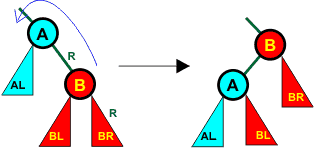
\includegraphics[width=0.8\linewidth]{avl-trees/rr-rotation.png}
        \columnbreak \\
        \textbf{Rotacja LL} \\

        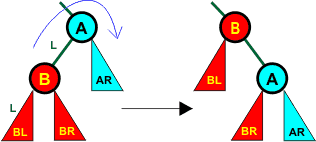
\includegraphics[width=0.8\linewidth]{avl-trees/ll-rotation.png}
    \end{multicols}

    \textbf{Rotacja RL} \\

    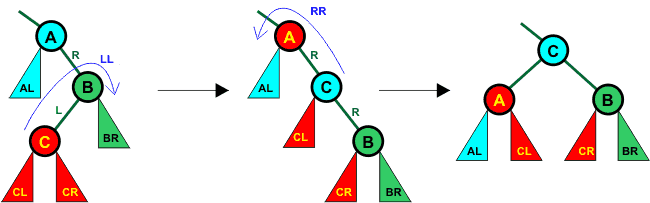
\includegraphics[width=\linewidth]{avl-trees/rl-rotation.png} \\

    \textbf{Rotacja LR} \\

    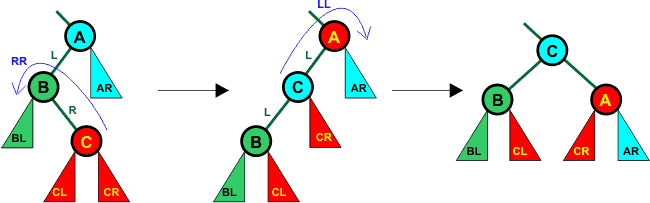
\includegraphics[width=\linewidth]{avl-trees/lr-rotation.png} \\

    \noindent Gdy \texttt{nierównowaga drzewa} idzie dwa razy na prawo (tzn. gdy dla danego węzła prawe poddrzewo jest głębsze niż lewe i potem dla pierwszego węzła prawego poddrzewa jego prawe poddrzewo jest głębsze) do zbalansowania używamy rotacji RR, natomiast, gdy nierównowaga idzie najpierw na prawo potem na lewo, używamy rotacji RL, itd.

    \newpage

    \section{Algorytmy przeszukiwania wszerz i w głąb w grafach.}

    Algorymy przeszukiwania grafu polegają na przejściu przez wszystkie osiągalne z wierzchołka
    startowego $s$ wierzchołki grafu $G$.

    \subsection{Przeszukiwanie grafu wszerz (\textit{breadth first search}, BFS)}

    \subsubsection{Algorytm}

    Do przeszukiwania użyjemy kolejki $Q = \{s\}$. Ponadto używamy koloru czarnego do
    oznaczania odwiedzonych już wierzchołków.\[\]
    Dopóki kolejka nie jest pusta:
    \begin{enumerate}
        \item Zdejm $x$ z kolejki
        \item Pomaluj $x$ na czarno
        \item Dla każdego niepomalowanego na czarno $v$, sąsiadującego z $x$ wrzuć
        $v$ do kolejki
    \end{enumerate}

    \subsubsection{Cechy}

    \begin{enumerate}
        \item Zlożoność obliczeniowa: $\theta(e + v)$
        \item Złożoność pamięciowa: $\theta(v)$
        \item Kompletność: BFS dla nieskończonego grafu zwróci wszystkie poprawne
        odpowiedzi, w przeciwieństwie do DFS.
    \end{enumerate}

    \subsubsection{Wariacje algorytmu}

    \begin{itemize}
        \item Faktyczne "przeszukiwanie": zwracamy wieszchołek, jeśli jego wartość jest
        równa poszukiwanej.
        \item Przypisywanie wierzchołkom odległości od $s$.
        \item Przypisanie wierzchołkom rodzica, w celu znalezienia drogi do $s$
    \end{itemize}

    \subsubsection{Zastosowania}

    \begin{itemize}
        \item Garbage collection
        \item Najkrótsza droga do $s$ (licząć liczbę krawędzi)
        \item Wykrywanie cykli grafu nieskierowanego
        \item Sprawdzanie dwudzielności grafu
        \item Social networking
        \item Algorytmy sieci przepływowych (np. wyznaczanie maksymalnego przepływu)
        \item Crawlery
    \end{itemize}

    \subsection{Przeszukiwanie grafu wgłąb (\textit{depth first search}, DFS)}

    \subsubsection{Algorytm}

    Używamy koloru czarnego do oznaczania odwiedzonych już wierzchołków.\[\]
    Dla danego wierzchołka $x$ (zaczynając od $s$):
    \begin{enumerate}
        \item Pomaluj $x$ na czarno
        \item Wywołaj się rekurencyjnie dla każdego niepomalowanego na czarno $v$,
        sąsiadującego z $x$
    \end{enumerate}


    \subsubsection{Wersja z zapamiętywaniem rodzica}

    Słownik $P = \{s : null\}$ przypisuje każdemu wierzchołkowi (poza $s$) rodzica. Używamy
    koloru czarnego do oznaczania odwiedzonych już wierzchołków, oraz szarego do
    wierzchołków właśnie odwiedzanych.\[\]
    Dla danego wierzchołka $x$ (zaczynając od $s$):
    \begin{enumerate}
        \item Pomaluj $x$ na szaro
        \item Dla każdego białego $v$, sąsiadującego z $x$:
        \begin{enumerate}
            \item $P[v] = x$
            \item Wywołaj się rekurencyjnie na $v$
        \end{enumerate}
        \item Pomaluj $x$ na czarno
    \end{enumerate}

    \subsubsection{Cechy}

    \begin{enumerate}
        \item Zlożoność obliczeniowa: $\theta(e + v)$
        \item Złożoność pamięciowa: $\theta(v)$
        \item Niekompletność dla grafów nieskończonych
    \end{enumerate}

    \subsubsection{Wariacje algorytmu}

    \begin{itemize}
        \item Faktyczne "przeszukiwanie": zwracamy wieszchołek, jeśli jego wartość jest
        równa poszukiwanej.
        \item Przypisywanie wierzchołkom odległości od $s$.
        \item Przypisanie wierzchołkom rodzica, w celu znalezienia drogi do $s$
    \end{itemize}

    \subsubsection{Zastosowania}

    \begin{itemize}
        \item Garbage collection
        \item Minimalne drzewo rozpinające (dla grafów nieważonych)
        \item Wykrywanie cykli w grafie skierowanym
        \item Sortowanie topologiczne
        \item Wykrywanie cykli grafu nieskierowanego
        \item Algorytmy sieci przepływowych (np. wyznaczanie maksymalnego przepływu)
        \item Crawlery
        \item Labirynty
    \end{itemize}

    \newpage

    \section{Algorytmy wyszukiwania najkrótszej ścieżki (Dijkstry oraz Bellmana-Forda).}

    W algorytmach wyszukiwania najkrótszej ścieżki używamy procedury \textit{relax(u, v, w)},
    sprawdzającej, czy ścieżka z $u$ do $w$ przez $v$ jest krótsza od aktualnie najkrótszej
    ścieżki.
    \\~\\
    \textit{relax(u, v, w)}:
    \vskip 0pt Jeśli $D[u, w] = D[u, v] + D[v, w]$ to:\\
    \hspace*{1cm} $D[u, w] = D[u, v] + D[v, w]$\\
    \hspace*{1cm} $P[u, w] = v$\\

    \subsection{Algorytm Dijkstry}

    Algorytm Dijkstry pozwala na wyliczenie w grafie $G = \{V, E\}$ najkrótszej ścieżki od wierzchołka
    startowego $s$ do wszystkich pozostałych wierzchołków. $|V| = v, |E| = e$

    \subsubsection{Algorytm}

    Posługujemy się słownikiem $P = \{\}$ przypisującym każdemu wierzchołkowi
    rodzica (w celu znalezienia ścieżki), słownikiem $D$ oznaczającym odległość
    wierzchołków od $s$ oraz kolejką priorytetową $S = \{v \in V : D[v]\}$ nieodwiedzonych
    wierzchołków. $D[s] = 0; D[\forall v \in V \setminus \{s\}] = \infty$.
    \[\]
    Używamy uproszczonej procedury \textit{relax} - wierzchołkiem startowym ($u$) jest zawsze $s$
    \[\]
    \textit{relax(v, w)}:
    \vskip 0pt Jeśli $D[w] = D[v] + e_{v \rightarrow w}$ to:\\
    \hspace*{1cm} $D[w] = D[v] + e_{v \rightarrow w}$ \\
    \hspace*{1cm} $P[w] = v$ \\

    \[\]
    Dopóki $S \neq \o$:
    \begin{enumerate}
        \item Usuń wierzchołek $v$ o najmniejszej wartości z $S$
        \item Dla każdego wierzchołka $w$ sąsiadującego z $v$ wywołaj \textit{relax(v, w)}
    \end{enumerate}

    \subsubsection{Złożoność}

    \begin{itemize}
        \item Inicjalizacja - $\theta(v)$
        \item $\theta(v)$ usunięć z kolejki
        \item $O(e)$ pomniejszeń wartości w $D$
        \item Przy pomocy kopca binarnego możemy uzyskać $O(\log(v))$ dla pomniejszenia
        wartości, $O(\log(v))$ dla usunięcia z kolejki. Złożoność:
        $\theta((e + v)\log(v))$

        \item Przy pomocy kopca Fibonacciego możemy uzyskać $\theta(1)$ dla pomniejszenia
        wartości, $\theta(\log (v))$ dla usunięcia z kolki. Złożoność:
        $O(v \cdot \log(v) + e)$
    \end{itemize}

    \subsubsection{Cechy}

    \begin{itemize}
        \item Nie działa poprawnie dla grafów z wagami ujemnymi
        \item Algorytm zachłanny
    \end{itemize}

    \subsection{Algorytm Bellmana-Forda}

    Algorytm Bellmana-Forda pozwala na wyliczenie w grafie $G$ najkrótszej ścieżki z
    wierzchołka startowego $s$ do wszystkich pozostałych wierzchołków.

    \subsubsection{Algorytm}

    Posługujemy się słownikiem $P = \{\}$, przypisującym każdemu wierzchołkowi
    rodzica (w celu znalezienia ścieżki), słownikiem $D$ oznaczającym odległość
    wierzchołków\\ od $s$. $D[s] = 0; D[v] = \infty \; \forall v \in V \setminus \{s\}$.
    \[\]
    Ponownie używamy uproszczonej procedury \textit{relax}.

    \[\]
    Dla każdego wierzchołka w $V \setminus \{s\}$:
    \vskip 0pt Wywołaj \textit{relax(u, v)} dla każdej krawędzi $(u, v) \in E$
    \[\]

    Dodatkowo można wykonać sprawdzenie, czy w grafie nie ma cykli o wadze ujemnej:

    \[\]
    Dla każdej krawędzi $(u, v) \in E$:
    \vskip 0pt Jeśli $D[v] > D[u] + e_{u \rightarrow v}$, to
    istnieje cykl o wadze ujemnej.
    \subsubsection{Złożoność}

    $O(v \cdot e)$

    \subsubsection{Cechy}

    \begin{itemize}
        \item Działa poprawnie dla grafów z wagami ujemnymi (bez cykli o wagach ujemnych)
        \item Pozwala decydować, czy graf ma cykle ujemne
        \item Używany w protokole RIP
        \item Algorytm można zoptymalizować: jeśli w danej iteracji nie dokonał zmiany,
        należy przerwać jego działanie (ścieżki już są najkrótsze)
    \end{itemize}

    \subsection{Algorytm Floyda-Warshalla}

    Algorytm Floyda-Warshalla pozwala wyliczyć najkrósze ścieżki pomiędzy wszystkimi
    wierzchołkami w grafie $G$ (nieposiadającym ujemnych cykli).

    \subsubsection{Algorytm}

    Posługujemy się słownikiem $P = \{\}$, przypisującym parze $(u, w)$ rodzica dla $u$,
    na ścieżce od $u$ do $w$, słownikiem $D$ przypisującym parze $(u, w)$ długość
    najkrószej (aktualnie) ścieżki od $u$ do $w$.\\
    $D[(u, w) : u, w \in V] =
    \begin{cases}
        0, &\text{ jeśli } u = w\\
        e_{u \rightarrow w}, &\text{ jeśli } (u, w) \in E\\
        \infty, &\text{ jeśli } (u, w) \notin E
    \end{cases}$.
    \[\]

    Wywołaj  \textit{relax(u, v, w)} dla każdej trójki $(u, v, w) : u, w, v \in V$ wywołaj
    \subsubsection{Złożoność}
    $\theta(v^3)$

    \subsubsection{Cechy}
    \begin{itemize}
        \item Prostota
        \item Pozwala obliczyć za jednym razem wszystkie ścieżki pomiędzy wierzchołkami
        \item Działa dla grafów z krawędziami ujemnymi (ale nie z cyklami ujemnymi)
        \item Złożoność jest niezależna od gęstości grafu
    \end{itemize}

    \section{Programowanie dynamiczne: podział na podproblemy, porównanie z metodą "dziel i zwyciężaj".}

    \begin{definition}
        \textbf{Programowanie dynamiczne}

        Technika projektowania algorytmów polegająca na \textbf{podziale problemu na mniejsze podproblemy} względem kilku parametrów (podobnie jak w metodzie dziel i zwyciężaj).

        Wyniki rozwiązywania podproblemów są  \textbf{zapisywane w tabeli}, dzięki czemu w przypadku natrafienia na ten sam podproblem nie trzeba go ponownie rozwiązywać.

        Cechy
        \begin{itemize}
            \item Problem posiada powtarzające się podproblemy
            \item Podproblemy musi cechować \textbf{własność optymalnej podstruktury}
            \item Zastosowanie brute force prowadzi do \textbf{ponadwielomianowej} liczby rozwiązań podproblemów, podczas gdy sama liczba różnych podproblemów jest wielomianowa
        \end{itemize}

        Niejednokrotnie stosowanie techniki programowania dynamicznego daje w rezultacie algorytm pseudowielomianowy.
    \end{definition}

    \begin{definition}
        \textbf{Własność optymalnej podstruktury}

        Oznacza, że optymalne rozwiązanie problemu jest \textbf{funkcją optymalnych rozwiązań podproblemów}, czyli znając optymalne rozwiązania podproblemów można efektywnie wyznaczyć rozwiązanie problemu.
    \end{definition}

    \begin{definition}
        \textbf{Funkcja celowa}

        W zadaniach programowania liniowego liniowa funkcja, dla której szukane jest optymalne rozwiązanie minimum lub maksimum. Dla zdefiniowanego zadania programowania liniowego

        Optymalizacja – problem polegający na znalezieniu ekstremum zadanej funkcji celu.
    \end{definition}

    Metody Programowania Dynamicznego
    \begin{itemize}
        \item Metoda zstępująca z zapamiętywaniem polega na rekurencyjnym wywoływaniu funkcji z zapamiętywaniem wyników. Metoda ta jest podobna do metody dziel i zwyciężaj – różni się od niej tym, że jeśli rozwiązanie danego problemu jest już w tabeli z wynikami, to należy je po prostu stamtąd odczytać.
        \item Metoda wstępująca polega na rozwiązywaniu wszystkich możliwych podproblemów, zaczynając od tych o najmniejszym rozmiarze. Wówczas w momencie rozwiązywania podproblemu na pewno są już dostępne rozwiązania jego podproblemów. W tym podejściu nie zużywa się pamięci na rekurencyjne wywołania funkcji. Może się jednak okazać, że część podproblemów została rozwiązana nadmiarowo (nie były one potrzebne do rozwiązania głównego problemu).
    \end{itemize}

    Klucz do zaprojektowania algorytmu tą techniką leży w znalezieniu \textbf{równania rekurencyjnego} opisującego optymalną wartość \textbf{funkcji celu} dla danego problemu jako funkcji optymalnych wartości funkcji celu dla podproblemów o mniejszych rozmiarach. Programowanie dynamiczne znajduje optymalną wartość funkcji celu dla całego zagadnienia, rozwiązując podproblemy od najmniejszego do największego i zapisując optymalne wartości w tablicy. Pozwala to zastąpić wywołania rekurencyjne odwołaniami do odpowiednich komórek wspomnianej tablicy i gwarantuje, że każdy podproblem jest rozwiązywany tylko raz. Rozwiązanie ostatniego z rozpatrywanych podproblemów jest na ogół wartością rozwiązania zadanego zagadnienia.

    Przykład - Ciąg Fibonacci'ego

    \begin{verbatim}
        # Programowanie dynamiczne wstępujące, wersja z listą.
        def fibonacci(n):
        F = [0] + n * [1]   # trzymamy wszystkie wartości
        for i in range(2, n+1):
        F[i] = F[i-1] + F[i-2]
        return F[n]
    \end{verbatim}

    \begin{verbatim}
        # Programowanie dynamiczne zstępujące.
        FIBONACCI = {0:0, 1:1}   # globalny słownik

        def fibonacci(n):
        global FIBONACCI
        if n not in FIBONACCI:
        FIBONACCI[n] = fibonacci(n-1) + fibonacci(n-2)
        return FIBONACCI[n]
    \end{verbatim}

    \newpage

    \section{Algorytm zachłanny: przykład optymalnego i nieoptymalnego wykorzystania.}

    \begin{definition}
        Algorytmy zachłanne (ang. greedy algorithms)

        Algorytmy podejmujące w każdym kroku taką decyzję, która w danej chwili jest najkorzystniejsza (\textbf{lokalnie optymalna}) licząc, że doprowadzi to do znalezienia rozwiązania \textbf{globalnie optymalnego}.

        Cechy

        \begin{itemize}
            \item Nie zawsze znajdują rozwiązanie optymalne
            \item Są podzbiorem algorytmów \textbf{heurystycznych}
            \item Są to algorytmy \textbf{deterministyczne} – nie ma w nich losowości
        \end{itemize}

    \end{definition}

    % Tu był przykład z wydawaniem reszty. Usuwam, bo ciężko zdefiniować "nieoptymalne" rozwiązanie - ktoś na egzaminie mógłby mieć przez to problem.

    Przykład - Pakowanie plecaka

    \begin{verbatim}
        posortuj nierosnąco przedmioty według wartości c[j]/w[j]
        aktualna_waga:=0

        for i:=1 to n do
        if w[i] + aktualna_waga <= W then
        dodaj i-ty przedmiot do plecaka
        aktualna_waga := aktualna_waga + w[i]
    \end{verbatim}

    Dane wejściowe, dla których algorytm będzie działał
    \begin{itemize}
        \item Optymalnie

        Pjemność plecaka: 8

        Dane wejściowe: 5, 3, 2, 1, 1, 1, 1, 1, 1, 1, 1

        Rozwiązanie: 5 + 3 + 2

        \item Nieoptymalnie

        Pojemność plecaka: 7

        Dane wejściowe: 3, 3, 2, 2

        Rozwiązanie: 3 + 3 = 6 :(

        Rozwiązanie optymalne: 3 + 2 + 2 = 7

    \end{itemize}

    \newpage

    \section{Kolorowania wierzchołkowe (grafów planarnych) i krawędziowe grafów, algorytmy i ich złożoności.}

    \subsection{Kolorowanie krawędziowe grafów}
    Problem kolorowania krawędzi, podobnie jak klasycznego kolorowania wierzchołków, jest NP-trudny – nie istnieją wielomianowe algorytmy kolorujące grafy zawsze w sposób optymalny.
    \\\\
    Przykład nieopytymalnego algorytmu kolorowania krawędziowego:
    \begin{enumerate}
        \item Użyj BFS (Breadth First Search - Przeszukiwanie wszerz) do poruszania się po grafie.
        \item Wybierz wierzchołek i nadaj różne kolory jego krawędziom.
        \item Przejdź do kolejnego wierzchołka.
        \item Powtarzaj aż wszyskie krawędzie zostaną pokolorowane.
    \end{enumerate}

    \subsection{Kolorowanie wierzchołkowe grafów planarnych}

    \begin{definition}
        Graf planarny - graf, który można narysować na płaszczyźnie tak, by krzywe obrazujące krawędzie grafu nie przecinały się ze sobą.
    \end{definition}

    \begin{theorem}
        Liczba chromatyczna grafu planarnego jest równa lub mniejsza niż 4
    \end{theorem}

    Każdy graf planarny można pokolorować 5 kolorami w czasie liniowym.





    \newpage

    \section{Algorytmy wyszukiwania minimalnego drzewa rozpinającego: Boruvki, Prima i Kruskala.}

    \subsection{Algorytm Boruvki}
    \begin{enumerate}
        \item Weź wszystkie wierzchołki, ale bez krawędzi - każdy wierzchołek jest osobnym drzewem.
        \item Dla każdego drzewa znajdź krawędź o najmniejszej wadze w oryignalnym grafie, która łączy je z innym drzewem.
        \item Dodaj tę krawędź do MST.
        \item Powtarzaj, dopóki drzewa nie połączyły się w jedno.
    \end{enumerate}
    \textbf{Złożoność:} $O(ElogV)$.


    \subsection{Algorytm Prima}
    \begin{enumerate}
        \item Zainicjalizuj MST jednym wierzchołkiem, wybranym losowo z grafu.
        \item Spośród krawędzi łączących MST z wierzchołkami jeszcze w nim niebędącymi wybierz tę, która ma najmniejszą wagę, i dodaj ją do MST.
        \item Powtarzaj krok 2 aż wszystkie wierzchołki znajdą się w MST.
    \end{enumerate}
    \textbf{Złożoność:} Zależy od użytych struktur danych. $O(V^2)$ lub $O(ElogV)$, jeśli użyta została lista sąsiedztwa.



    \subsection{Algorytm Kruskala}

    \begin{enumerate}
        \item Posortuj krawędzie niemalejąco pod względem wag.
        \item Wybierz krawędź o najmniejszej wadze. Sprawdź czy tworzy cykl z MST utworzonym do tej pory. Jeśli nie, uwzględnij tą krawędź w MST. W przeciwnym wypadku, odrzuć.
        \item Powtarzaj krok 2 aż otrzymasz $V-1$ krawędzi w MST
    \end{enumerate}

    \textbf{Złożoność:} Sortowanie krawędzi zajmuje $O(ElogE)$. Po sortowaniu, iterujemy po krawędziach i używamy algorytmu find-union który może zająć $O(logV)$. Zatem ogólna złozoność to $O(ElogE+ElogV)$. Wartość E jest mniejsza niż $V^2$, więc $O(logV)$ $=$ $O(logE)$. Złożoność: $O(ElogE)$ lub $O(ElogV)$.

    \newpage

    \section{Najważniejsze algorytmy wyznaczania otoczki wypukłej zbioru punktów w układzie współrzędnych (Grahama, Jarvisa, algorytm przyrostowy (quickhull)).}

    \begin{definition}
        \textbf{Algorytm Grahama} - złożoność $O(n \log n)$.
        \begin{enumerate}
            \item Wybierz punkt (ozn. O) o najmniejszym y (jeśli jest kilka ex aequo, to ten z nich o najmniejszym x).
            \item Posortuj pozostałe punkty leksykograficznie względem:
            \begin{itemize}
                \item kąta pomiędzy wektorem $OP_i$ a osią X,
                \item długości wektora $OP_i$.
            \end{itemize}
            \item Przeglądaj listę posortowanych punktów:
            \begin{itemize}
                \item Od bieżącej pozycji weź trzy kolejne punkty (ozn. A, B, C).
                \item Jeśli punkt B leży na zewnątrz trójkąta AOC, to może należeć do otoczki wypukłej. Przejdź do następnej trójki punktów.
                \item Jeśli punkt B leży wewnątrz trójkąta AOC, to znaczy, że nie należy do otoczki. Usuń punkt B z listy i cofnij się o jedną pozycję (o ile bieżąca pozycja jest różna od początkowej).
            \end{itemize}
            \item Pozostałe na liście punkty stanowią otoczkę wypukłą.
        \end{enumerate}
    \end{definition}

    \begin{definition}
        \textbf{Algorytm Jarvisa} - średnia złożoność $O(kn)$, gdzie n - liczba punktów, k - liczba punktów należących do otoczki; pesymistyczna - $O(n^2)$.
        \begin{enumerate}
            \item $P_1$ – punkt na otoczce wypukłej o najmniejszej współrzędnej y (jeśli jest więcej niż jeden, wybierany jest ten o najmniejszej współrzędnej x),
            \item $P_{0}:=[-\infty ,y(P_{1})]$,
            \item $i:=1$,
            \item powtarzaj:
            \begin{itemize}
                \item $P_{i+1}$ – punkt $N$, dla którego kąt $P_{i-1}P_{i}N$ jest największy,
                \item jeśli $N=P_{1}$, koniec iterowania,
                \item $i:=i+1$,
            \end{itemize}
            \item ostatecznie otoczkę tworzą punkty $P_{1\dots i}$.
        \end{enumerate}

        Implementację można usprawnić, odrzucając w każdej iteracji punkty znajdujące się po prawej stronie wektora $P_{1}P_{i}$, ponieważ na pewno nie będą należały do otoczki. Zabieg ten nie wpływa jednak na asymptotyczną złożoność obliczeniową algorytmu.
    \end{definition}

    \begin{definition}
        \textbf{Quickhull} - średnia złożoność $O(n \log n)$, pesymistyczna złożoność - $O(n^2)$.

        QuickHull(P):
        \begin{enumerate}
            \item Znajdź w $P$ punkty o minimalnym i maksymalnym x (A oraz B).
            \item Podziel $P$ na dwa podzbiory $S_1$ i $S_2$ znajdujące się nad i pod prostą $AB$.
            \item Wywołaj rekurencyjnie QuickHull(A, B, $S_1$) i QuickHull(B, A, $S_2$).
        \end{enumerate}

        QuickHull(A, B, P) - funkcja pomocnicza:
        \begin{enumerate}
            \item Jeśli $P$ jest pusty – koniec.
            \item Jeśli $P$ ma jeden element, ten punkt należy do otoczki – koniec.
            \item W przeciwnym razie:
            \begin{itemize}
                \item Znajdź w $P$ punkt $C$ najbardziej oddalony od prostej $AB$. Ten punkt należy do otoczki wypukłej.
                \item Odrzuć wszystkie punkty z wnętrza trójkąta $ABC$, nie mogą należeć do otoczki.
                \item Znajdź zbiór $S_1$ punktów znajdujących się po prawej stronie prostej $AC$C oraz analogiczny
                zbiór $S_2$ dla prostej $BC$. (Stronę określa znak równania ogólnego prostej).
                \item Wywołaj rekurencyjnie QuickHull(A, C, $S_1$) i QuickHull(B, C, $S_2$).
            \end{itemize}
        \end{enumerate}
    \end{definition}

    \newpage

    \section{Problemy P, NP, NP-zupełne i zależności między nimi. Hipoteza P vs. NP.}
    \begin{definition}
        \textbf{Problem P} (ang. \textit{deterministic polynomial}, deterministycznie wielomianowy) – problem decyzyjny,
        dla którego rozwiązanie można \textbf{znaleźć} w czasie wielomianowym.
    \end{definition}

    \begin{definition}
        \textbf{Problem NP} (ang. \textit{nondeterministic polynomial}, niedeterministycznie wielomianowy) – problem
        decyzyjny, dla którego rozwiązanie można \textbf{zweryfikować} w czasie wielomianowym.
    \end{definition}

    \begin{theorem}
        $\mathbf{P \stackrel{?}{=} NP}$. Każdy problem P jest NP, jednak nie wiadomo czy istnieje problem NP niebędący P.
    \end{theorem}

    \begin{definition}
        \textbf{Problem NP-zupełny} (ang. \textit{NP-Complete}) – taki problem \textbf{NP}, do którego można \textbf{w czasie wielomianowym zredukować} dowolny inny problem NP. Czasami zamiast redukcji w czasie wielomianowym używa się redukcji w pamięci logarytmicznej.
    \end{definition}
    Stąd wynika, że jeśli potrafimy rozwiązać jakikolwiek problem NP-zupełny w czasie wielomianowym,
    to potrafimy rozwiązać w takim czasie wszystkie problemy NP.

    \newpage

    \section{Automat minimalny, wybrany algorytm minimalizacji.}
    \subsection{Automat minimalny}
    \begin{definition}
        Automat $\mathcal{A} = (S, A, f, s_{0}, T)$ rozpoznający język L jest minimalny, jeśli posiada najmniejszą liczbę stanów spośród wszystkich automatów rozpoznających język L.
    \end{definition}

    \begin{definition}
        Dla dowolnego języka $L \in \mathcal{REC}(A^{*})$ automat
        \begin{center}
            $\mathcal{A}_{P_{L}^{r}} = (A^{*} / P_{L}^{r}, A, f^{*}, [1]_{P_{L}^{r}}, T)$,
        \end{center}
        gdzie $T = \{[w]_{P_{L}^{r}} : w \in L \}$ jest automatem minimalnym rozpoznającym język L
    \end{definition}
    \begin{definition}
        \textbf{Konstrukcja automatu minimalnego z wykorzystaniem prawej kongruencji automatowej} \\
        $L \subset A^{*}$ - dowolny język \\
        $\Theta_{L} \subset A^* \times A^*$ - relacja równoważności dzieląca $A^*$ na dwie klasy:
        \begin{center}
            L oraz $A^* \setminus L$
        \end{center}
        $\rho_i$ dla $i \in \mathbb{N}$ - zstępujący ciąg relacji: \\
        $\rho_1 = \Theta_L$, \\
        $\rho_i = \{(u, w) \in A^* \times A^* : \forall a \in A \cup \{\textbf{1}\}: (ua, wa) \in \rho_{i-1} \}$ dla i = 2, \ldots \\
        Wtedy
        \begin{center}
            $\bigcap\limits_{i \in \mathbb{N}} \rho_i = P^r_L$
        \end{center}
    \end{definition}


    \subsection{Minimalizacja automatu}
    \begin{definition}
        \textbf{Algorytm ``Minimalizuj 1''} \\
        \url{http://wazniak.mimuw.edu.pl/index.php?title=J\%C4\%99zyki\%2C_automaty_i_obliczenia/Wyk\%C5\%82ad_5:_Algorytmy_konstrukcji_automatu_minimalnego} \\
        Wejście L - język \\
        Wyjście: automat minimalny $\mathcal{A} = (S_L, A, f_F, s_L, T_L)$ taki, że $L\mathcal{A} = L$
        \begin{lstlisting}
            $S_L \leftarrow \{L\};$
            Put$(\mathcal{L}, L);$
            while $\mathcal{L} \neq \emptyset$ do
            M $\leftarrow$ \textbf{zdejmij} $(\mathcal{L})$;
            foreach $a \in A$ do
            N $\leftarrow a^{-1}M$;
            if $N \cap S_L = \emptyset$ then
            $S_L \leftarrow S_L \cup \{N\}$;
            Put$(\mathcal{L}, N);$
            end if
            end for
            end while
            foreach $M \in S_L$ do
            foreach $a \in A$ do
            $f_L(M, a) \leftarrow a^{-1}M$;
            end for
            end for
            $s_L \leftarrow L$;
            $T_L \leftarrow \{u^{-1}L : u \in L\}$;
            return $\mathcal{A}'$;
        \end{lstlisting}
    \end{definition}

    \section{Lemat o pompowaniu dla języków regularnych.}
    \begin{definition}
        Niech $L \subset A^*$ będzie językiem rozpoznawalnym. Istnieje liczba naturalna $N \geq 1$ taka, że dowolne słowo $w \in L$ o długości $|w| \geq N$ można rozłożyć na katenację:
        \begin{center}
            $w = v_1 u v_2$
        \end{center}
        gdzie $v_1, v_2 \in A^*, u \in A^+, |v_1 u| < N$ oraz
        \begin{center}
            $v_1 u^* v_2 \subset L$
        \end{center}
    \end{definition}

    \begin{definition}
        Jeśli rozpoznawalny język $L \subset A^*$ jest nieskończony, to istnieją
        $v_1, v_2 \in A^*, u \in A^+$, takie, że
        \begin{center}
            $v_1 u^* v_2 \subset L$
        \end{center}
    \end{definition}

    \newpage

    \section{Warunki równoważne definicji języka regularnego: automat, prawa kongruencja syntaktyczna, wyrażenia regularne.}
    \subsection{Wyrażenia regularne}

    \begin{definition}
        \textbf{Rodzina regularnych podzbiorów}

        Niech $A$ będzie dowolnym zbiorem. Rodzina $REG(A^*)$ regularnych podzbiorów
        $A^*$ to najmniejsza rodzina $R$ podzbiorów $A^*$ taka, że:

        \begin{enumerate}
            \item $\emptyset \in R, \forall a \in A$ ${a} \in R$
            \item jeśli $X, Y \in R$, to: $X \cup Y, X \cdot Y \in R$
            \item jeśli $X \in R$, to: $X^* = \bigcup\limits_{n = 0}^{\infty} X^n \in R$
        \end{enumerate}
    \end{definition}

    \begin{definition}
        \textbf{Wyrażenie regularne}

        Niech $A$ będzie dowolnym alfabetem, a zbiór $\{+, \star, \emptyset, (,)\}$
        alfabetem takim, że $A \cap \{+, \star, \emptyset, (,)\} = \emptyset$.

        Słowo $\alpha \in (A \cup \{+, \star, \emptyset, (,)\})^*$ jest wyrażeniem regularnym
        nad alfabetem A wtedy i tylko wtedy, gdy:

        \begin{enumerate}
            \item $\alpha = \emptyset$
            \item $\alpha = a \in A$
            \item $\alpha$ jest w postaci $(\beta + \gamma), (\beta\gamma), \gamma^*$, gdzie
            $\beta, \gamma$ są wyrażeniami regularnymi nad alfabetem A
        \end{enumerate}
    \end{definition}

    Rodzinę wyrażeń regularnych nad $A$ nazywamy $WR$.

    \subsection{Automat skończony}

    \begin{definition}
        \textbf{Automat}

        Automatem nad alfabetem A nazywamy system $\mathcal{A} = (S, f)$ w którym:
        \begin{itemize}
            \item S jest dowolnym zbiorem, zwanym zbiorem stanów
            \item $f : S \times A \rightarrow S$ jest funkcją przejść
        \end{itemize}

        Automat $\mathcal{A}$ nazywamy skończonym, jeśli zbiór S jest skończony

        Automat $\mathcal{A}$ ze stanem $s \in S$ taki, że
        \[f(a, A^*) = Ss\]
        nazywamy automatem z generatorem s.
    \end{definition}

    \begin{definition}
        \textbf{Język rozpoznawalny}

        Język $L \subset A^*$ jest rozpoznawalny wtedy i tylko wtedy, gdy istnieją:
        \begin{itemize}
            \item Automat skończony $\mathcal{A} = (S, f)$
            \item stan $s_0 \in S$
            \item zbiór $T \subset S$
        \end{itemize}

        takie, że
        \[ L = \{w \in A^* : f(s_0, w) \in T\}\]
        $s_0$ - stan początkowy \\
        T - zbiór stanów końcowych automatu
        \[\mathcal{A} = (S, A, f, s_0, T)\]
        $L = L(\mathcal{A})$ - język rozpoznawany przez automat $\mathcal{A}$\\
        $REC(A^*)$ - rodzina wszystkich języków rozpoznawalnych nad alfabetem A
    \end{definition}

    \subsection{Prawa kongruencja syntaktyczna}

    \begin{definition}
        \textbf{Prawa kongruencja}

        Każdy automat $\mathcal{A} = (S, f)$ z generatorem $s_0$ wyznacza na wolnym
        monoidzie $A^*$ prawą kongruencję $\sim_\mathcal{A}$:
        \[\]
        $\forall u, v \in A^*$
        \[u \sim_\mathcal{A} v \Leftrightarrow f(s_0, u) = f(s_0, v)\]

        Relacja $\sim_{\mathcal{A}}$ ma skończony indeks wtedy i tylko wtedy, gdy automat
        $\mathcal{A}$ jest skończony.
    \end{definition}

    \begin{theorem}
        Każda prawa kongruencja $p \subset (A^*)^2$ wyznacza automat, zwany ilorazowym
        \[\mathcal{A}_p = (A^* /_{p}, f^*), \; \mathrm{gdzie} \; f^*([w]_p, u) = [wu]_p\]
        \begin{itemize}
            \item $\mathcal{A}_p$ jest automatem z generatorem [1]$_p$

            \item $\mathcal{A}_p$ jest automatem skończonym wtedy i tylko gdy relacja $p$ ma skończony indeks
        \end{itemize}
    \end{theorem}

    \subsection{Warunki równoważne definicji języka regularnego}
    \begin{theorem}
        \textbf{Twierdzenie Kleenego}

        Dla każdego skończonego alfabetu A
        \[REC(A^*) = REG(^*)\]
    \end{theorem}

    \begin{theorem}
        Dla dowolnego języka regularnego $L \in A^*$ następujące warunki są równoważne:
        \begin{itemize}
            \item L = L(G) dla gramatyki G typu 3 (regularnej, lewoliniowej)
            \item L = L(G) dla gramatyki G prawoliniowej
            \item L = L($\mathcal{A}$) dla automatu deterministycznego $\mathcal{A}$
            \item L = L($\mathcal{A}_{ND}$) dla automatu niedeterministycznego $\mathcal{A}_{ND}$
            \item L = L($\mathcal{A}_{ND}$) dla automatu niedeterministycznego $\mathcal{A}_{ND}^p$ z pustymi przejściami

            \item L = $\|\alpha\|$ dla wyrażenia regularnego $\alpha$ nad alfabetem A
            \item L $\in REG(A^*)$
            \item monoid syntaktyczna M(L) jest skończony
            \item liczba różnych pochodnych Brzozowskiego dla języka
            L jest skończona
            \item L jest sumą wybranych klas równoważności pewnej prawej kongruencji na $A^*$
            o skończonym indeksie oraz L = $\bigcup\limits_{w \in L}[w]_p$
            \item istnieje skończony monoid M i homomorfizm
            \[\varphi : A^* \rightarrow M : L = \varphi^{-1}(\phi(L))\]
        \end{itemize}
    \end{theorem}

    \newpage
    \subsection{Konstrukcja automatu skończenie stanowego rozpoznającego wyrażenie regularne.}
    \begin{itemize}
        \item automat rozpoznający język pusty
        \begin{center}
            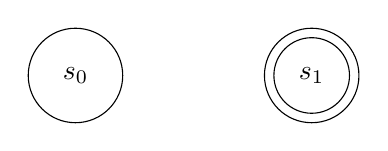
\begin{tikzpicture}[scale=0.2]
                \tikzstyle{every node}+=[inner sep=0pt]
                \draw [black] (13,-27) circle (3);
                \draw (13,-27) node {$s_0$};
                \draw [black] (28,-27) circle (3);
                \draw (28,-27) node {$s_1$};
                \draw [black] (28,-27) circle (2.4);
            \end{tikzpicture}
        \end{center}


        \item automat rozpoznający język $\{1\}$
        \begin{center}
            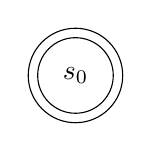
\begin{tikzpicture}[scale=0.2]
                \tikzstyle{every node}+=[inner sep=0pt]
                \draw [black] (29.4,-17.1) circle (3);
                \draw (29.4,-17.1) node {$s_0$};
                \draw [black] (29.4,-17.1) circle (2.4);
            \end{tikzpicture}
        \end{center}

        \item automat rozpoznający język $\{a\} \; \forall a \in A$
        \begin{center}
            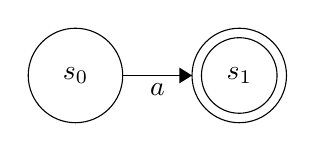
\begin{tikzpicture}[scale=0.2]
                \tikzstyle{every node}+=[inner sep=0pt]
                \draw [black] (29.4,-17.1) circle (3);
                \draw (29.4,-17.1) node {$s_0$};
                \draw [black] (39.8,-17.1) circle (3);
                \draw (39.8,-17.1) node {$s_1$};
                \draw [black] (39.8,-17.1) circle (2.4);
                \draw [black] (32.4,-17.1) -- (36.8,-17.1);
                \fill [black] (36.8,-17.1) -- (36,-16.6) -- (36,-17.6);
                \draw (34.6,-17.6) node [below] {$a$};
            \end{tikzpicture}
        \end{center}

        \newpage
        \item dla automatu $\mathcal{A}_r$ rozpoznającego wyrażenie $r$ i automatu $\mathcal{A}_r$ rozpoznającego wyrażenie $s$:
        $L(\mathcal{A}_x) = L(r + s)$ \\
        \noindent $\mathcal{A}_r = (S_r, A, f_r, s_{0r}, T_r) $ \\
        \noindent $\mathcal{A}_s = (S_s, A, f_s, s_{0s}, T_s) $ \\
        \noindent $\mathcal{A}_x = (S_x, A, f_x, s_{0x}, T_x) $ \\

        \[\mathcal{A}_s:\]
        \begin{center}
            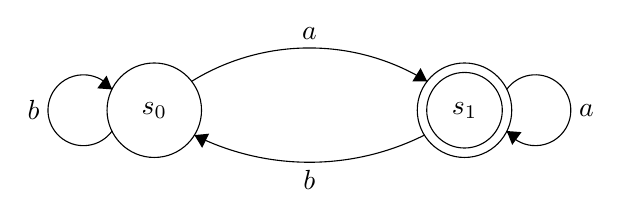
\begin{tikzpicture}[scale=0.2]
                \tikzstyle{every node}+=[inner sep=0pt]
                \draw [black] (18.2,-15.6) circle (3);
                \draw (18.2,-15.6) node {$s_0$};
                \draw [black] (37.9,-15.6) circle (3);
                \draw (37.9,-15.6) node {$s_1$};
                \draw [black] (37.9,-15.6) circle (2.4);
                \draw [black] (20.569,-13.768) arc (121.67786:58.32214:14.246);
                \fill [black] (35.53,-13.77) -- (35.11,-12.92) -- (34.59,-13.77);
                \draw (28.05,-11.15) node [above] {$a$};
                \draw [black] (35.355,-17.18) arc (-63.43003:-116.56997:16.331);
                \fill [black] (20.75,-17.18) -- (21.24,-17.99) -- (21.68,-17.09);
                \draw (28.05,-19.4) node [below] {$b$};
                \draw [black] (40.58,-14.277) arc (144:-144:2.25);
                \draw (45.15,-15.6) node [right] {$a$};
                \fill [black] (40.58,-16.92) -- (40.93,-17.8) -- (41.52,-16.99);
                \draw [black] (15.52,-16.923) arc (324:36:2.25);
                \draw (10.95,-15.6) node [left] {$b$};
                \fill [black] (15.52,-14.28) -- (15.17,-13.4) -- (14.58,-14.21);
            \end{tikzpicture}
        \end{center}


        \[\mathcal{A}_r:\]
        \begin{center}
            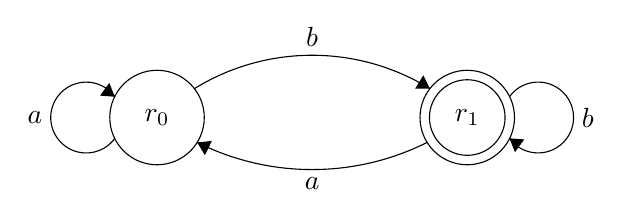
\begin{tikzpicture}[scale=0.2]
                \tikzstyle{every node}+=[inner sep=0pt]
                \draw [black] (18.2,-15.6) circle (3);
                \draw (18.2,-15.6) node {$r_0$};
                \draw [black] (37.9,-15.6) circle (3);
                \draw (37.9,-15.6) node {$r_1$};
                \draw [black] (37.9,-15.6) circle (2.4);
                \draw [black] (20.569,-13.768) arc (121.67786:58.32214:14.246);
                \fill [black] (35.53,-13.77) -- (35.11,-12.92) -- (34.59,-13.77);
                \draw (28.05,-11.15) node [above] {$b$};
                \draw [black] (35.355,-17.18) arc (-63.43003:-116.56997:16.331);
                \fill [black] (20.75,-17.18) -- (21.24,-17.99) -- (21.68,-17.09);
                \draw (28.05,-19.4) node [below] {$a$};
                \draw [black] (40.58,-14.277) arc (144:-144:2.25);
                \draw (45.15,-15.6) node [right] {$b$};
                \fill [black] (40.58,-16.92) -- (40.93,-17.8) -- (41.52,-16.99);
                \draw [black] (15.52,-16.923) arc (324:36:2.25);
                \draw (10.95,-15.6) node [left] {$a$};
                \fill [black] (15.52,-14.28) -- (15.17,-13.4) -- (14.58,-14.21);
            \end{tikzpicture}
        \end{center}


        \begin{itemize}
            \item automat rozpoznający język $r + s$:\\
            \noindent $s_{0x} = \{s_{0s}, s_{0r}\}$ \\
            \noindent $S_x = S_s \times S_r$ \\
            \noindent $f_x(\{s, r\}, a) = \{f_s(s, a), f_r(r, a)\}$ \\
            \noindent $T_x \ni t_x = \{s, r\} \Leftrightarrow s \in T_s \lor r \in T_R$ \\
            \begin{center}
                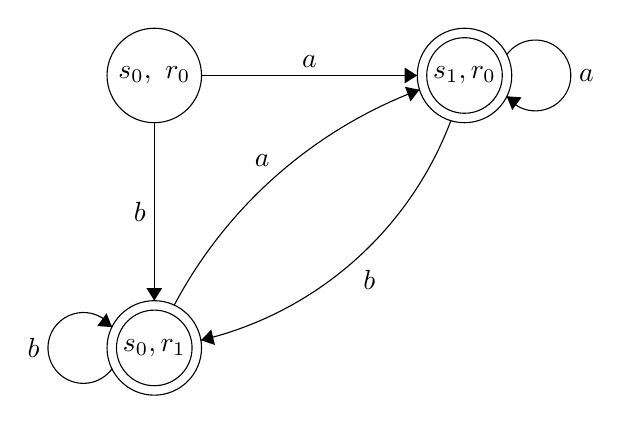
\begin{tikzpicture}[scale=0.2]
                    \tikzstyle{every node}+=[inner sep=0pt]
                    \draw [black] (18.2,-15.6) circle (3);
                    \draw (18.2,-15.6) node {$s_0,\mbox{ }r_0$};
                    \draw [black] (37.9,-15.6) circle (3);
                    \draw (37.9,-15.6) node {$s_1,r_0$};
                    \draw [black] (37.9,-15.6) circle (2.4);
                    \draw [black] (18.2,-32.9) circle (3);
                    \draw (18.2,-32.9) node {$s_0,r_1$};
                    \draw [black] (18.2,-32.9) circle (2.4);
                    \draw [black] (21.2,-15.6) -- (34.9,-15.6);
                    \fill [black] (34.9,-15.6) -- (34.1,-15.1) -- (34.1,-16.1);
                    \draw (28.05,-15.1) node [above] {$a$};
                    \draw [black] (18.2,-18.6) -- (18.2,-29.9);
                    \fill [black] (18.2,-29.9) -- (18.7,-29.1) -- (17.7,-29.1);
                    \draw (17.7,-24.25) node [left] {$b$};
                    \draw [black] (40.58,-14.277) arc (144:-144:2.25);
                    \draw (45.15,-15.6) node [right] {$a$};
                    \fill [black] (40.58,-16.92) -- (40.93,-17.8) -- (41.52,-16.99);
                    \draw [black] (15.52,-34.223) arc (324:36:2.25);
                    \draw (10.95,-32.9) node [left] {$b$};
                    \fill [black] (15.52,-31.58) -- (15.17,-30.7) -- (14.58,-31.51);
                    \draw [black] (19.468,-30.182) arc (152.05115:110.52628:29.234);
                    \fill [black] (35.04,-16.51) -- (34.12,-16.32) -- (34.47,-17.25);
                    \draw (25.05,-21.43) node [above] {$a$};
                    \draw [black] (37.033,-18.47) arc (-20.6381:-76.78447:22.448);
                    \fill [black] (21.16,-32.41) -- (22.05,-32.71) -- (21.82,-31.74);
                    \draw (31.85,-27.91) node [below] {$b$};
                \end{tikzpicture}
            \end{center}

            \item automat rozpoznający język $sr$:\\
            \noindent $s_{0x} = \{s_{0s}, \emptyset\}$ \\
            \noindent $S_x = (S_s \times \mathcal{P}(S_r))$\\
            \noindent $f_x(\{s, rs\}, a) = \{s_t, \bigcup\limits_{r \in rs}f_r(r)\}$ \\
            \noindent $f_s(s, a) = s_t \in T_s \rightarrow f_x(\{s, rs\}) = \{f_s(s, a), \{r_0\} \cup \bigcup\limits_{r \in rs}f_r(r, a)\}  $ \\
            \noindent $\{s, rs\} = t_x \in T_x \Leftrightarrow rs \cap T_r \neq \emptyset$ \\
            \begin{center}
                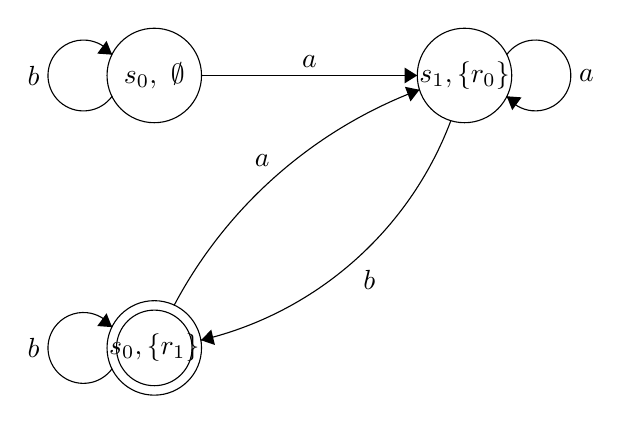
\begin{tikzpicture}[scale=0.2]
                    \tikzstyle{every node}+=[inner sep=0pt]
                    \draw [black] (18.2,-15.6) circle (3);
                    \draw (18.2,-15.6) node {$s_0,\mbox{ }\emptyset$};
                    \draw [black] (37.9,-15.6) circle (3);
                    \draw (37.9,-15.6) node {$s_1,\{r_0\}$};
                    \draw [black] (18.2,-32.9) circle (3);
                    \draw (18.2,-32.9) node {$s_0,\{r_1\}$};
                    \draw [black] (18.2,-32.9) circle (2.4);
                    \draw [black] (21.2,-15.6) -- (34.9,-15.6);
                    \fill [black] (34.9,-15.6) -- (34.1,-15.1) -- (34.1,-16.1);
                    \draw (28.05,-15.1) node [above] {$a$};
                    \draw [black] (40.58,-14.277) arc (144:-144:2.25);
                    \draw (45.15,-15.6) node [right] {$a$};
                    \fill [black] (40.58,-16.92) -- (40.93,-17.8) -- (41.52,-16.99);
                    \draw [black] (15.52,-34.223) arc (324:36:2.25);
                    \draw (10.95,-32.9) node [left] {$b$};
                    \fill [black] (15.52,-31.58) -- (15.17,-30.7) -- (14.58,-31.51);
                    \draw [black] (19.468,-30.182) arc (152.05115:110.52628:29.234);
                    \fill [black] (35.04,-16.51) -- (34.12,-16.32) -- (34.47,-17.25);
                    \draw (25.05,-21.43) node [above] {$a$};
                    \draw [black] (37.033,-18.47) arc (-20.6381:-76.78447:22.448);
                    \fill [black] (21.16,-32.41) -- (22.05,-32.71) -- (21.82,-31.74);
                    \draw (31.85,-27.91) node [below] {$b$};
                    \draw [black] (15.52,-16.923) arc (-36:-324:2.25);
                    \draw (10.95,-15.6) node [left] {$b$};
                    \fill [black] (15.52,-14.28) -- (15.17,-13.4) -- (14.58,-14.21);
                \end{tikzpicture}
            \end{center}

            \item automat rozpoznający język $r^*$:
            \noindent $s_{0x} = s_{0r}$\\
            \noindent $f_x(r, a) = f_r(r)$ \\
            \noindent $f_x(r_t \in R_t, 1) = r_{0x}$ \\
            \noindent $T_x = r_{0x}$ \\
        \end{itemize}
    \end{itemize}
    \newpage

    \section{Automaty niedeterministyczne i deterministyczne (w tym ze stosem); determinizacja.}

    \subsection{Determinizacja automatów skończenie stanowych}

    \begin{theorem}
        Język $L \in A^*$ jest rozpoznawany przez automat deterministyczny wtedy
        i tylko wtedy, gdy jest rozpoznawany przez automat niedeterministyczny.
    \end{theorem}

    $\mathcal{A}_{ND} = (S, f, I, F)$ - automat niedeterministyczny\\
    \indent$\mathcal{A}_D = (P(S), \overline{f}, I, T)$ - równoważny automat deterministyczny, gdzie:
    \begin{gather*}
        \overline{f} : P(S) \times A^* \rightarrow P(S)\\
        \forall Q \in P(S), \forall w \in A^* \; \; \overline{f}(Q, w) = \bigcup\limits_{s \in Q} f(s, w)\\
        T = \{Q \in P(S) | Q \cap F \neq \emptyset\}\\
    \end{gather*}

    \subsection{Determinizm automatu ze stosem}

    \begin{definition}
        \textbf{Deterministyczny automat ze stosem}

        Automatem $\mathcal{AS} = (A, A_S, Q, q_0, z_0, f, Q_F)$ nazywamy
        \textbf{deterministycznym}, jeśli dla każdej konfiguracji
        $(z, q, a) \in A_S^* \times Q \times (A \cup \{1\})$
        \begin{gather*}
            \# f(z, q, a) \leq 1 \; \mathrm{oraz}\\
            f(z, q, 1) \neq \emptyset \Rightarrow f(z, q, a) = \emptyset \; \forall a \in A\\
        \end{gather*}
        Język akceptowany przez automat deterministyczny nazywamy językiem deterministycznym.
    \end{definition}

    \begin{theorem}
        Każdy język deterministyczny jest jednoznaczny (rozpoznawany przez gramatykę jednoznaczną), ale nie na odwrót.
    \end{theorem}

    \begin{theorem}
        Każdy język deterministyczny jest kontekstowy (rozpoznawany przez niedeterministyczny automat ze stosem), ale nie na odwrót.
    \end{theorem}

    \newpage

    \section{Problemy rozstrzygalne i nierozstrzygalne w teorii języków.}

    Problemy rozpatrywane w kategorii języków
    \begin{itemize}
        \item Należenie $\in$ - Problem przynależności języka $L$ do jednego z typów języków $L_i$ gdzie $i \in {0,1,2,3}$ generowanych przez odpowiednie gramatyki  $G_i$
        \item Inkluzja $\subset$ - Problem zawierania się języka $L_i$ w języku $L_k$
        \item Równoważność $\equiv$ - Problem równoważności dwóch języków $L_1 \equiv L_2$
        \item Pustość $\emptyset$ - Problem języka pustego czyli nie generującego żadnego słowa
        \item Nieskończonośc $\infty$ - Problem języka nieskończonego czyli generującego nieskończenie wiele słów
        \item Jednoznaczność
    \end{itemize}

    \begin{definition}
        Wyprowadzenie lewostronne (prawostronne)

        Niech $G = (V_N,V_T,v_0,P)$ będzie gramatyką bezkontekstową.

        Lewostronnym (prawostronnym) wyprowadzeniem słowa $w \in {V_T}^\star$ w gramatyce $G$ nazywamy wyprowadzenie
        $v_0 \mapsto w_1 \mapsto \ldots.. \mapsto w_n = w$
        takie, że dla każdego $i=0,\ldots,n-1, \;\; w_{i+1}$ jest generowane bezpośrednio z $w_i$ przez zastąpienie pierwszego z lewej (prawej) symbolu nieterminalnego występującego w słowie $w_i$.
        Jeśli chcemy zaznaczyć, że wyprowadzenie jest lewostronne lub prawostronne, to posługujemy się zapisem

        $v_{0}\mapsto_{L}^{*}w,\; v_{0}\mapsto_{P}^{\star}w$.
    \end{definition}

    \begin{definition}
        Jednoznaczność -

        Gramatyka bezkontekstowa $G$ jest \textbf{jednoznaczna} $\Leftrightarrow$ każde słowo generowane przez tę gramatykę ma \textbf{dokładnie jedno wyprowadzenie lewostronne (prawostronne)}.

        Język bezkontekstowy $L$ nazywamy \textbf{jednoznacznym}, jeśli istnieje jednoznaczna gramatyka bezkontekstowa generująca ten język.

        Jednoznaczność gramatyki oznacza istnienie dokładnie jednego drzewa wywodu dla każdego generowanego słowa.
    \end{definition}


    \begin{center}
        \begin{tabular}{||c c c c c||}
            \hline
            --- & 3 & 2 & 1 & 0 \\ [0.5ex]
            \hline\hline
            Należenie $\in$ & T & T & T & N \\
            \hline
            Inkluzja $\subset$ & T & N & N & N \\
            \hline
            Równoważność $\equiv$ & T & N & N & N \\
            \hline
            Pustość $\emptyset$ & T & T & N & N \\
            \hline
            Nieskończoność $\infty$ & T & T & N & N \\
            \hline
            Jednoznaczność & T & N & - & - \\ [1ex]
            \hline
        \end{tabular}
    \end{center}

    Oznaczenia\\
    T - rozstrzygalny\\
    N - nieroztrzygalny

    \newpage


    \section{Klasy języków w hierarchii Chomsky’ego oraz ich zamkniętość ze względu na operacje boolowskie, homomorfizmy, itp.}

    \begin{definition}
        Gramatyka

        Jest to system $G=(V_N,V_T,P,v_0)$, w którym
        \begin{itemize}
            \item
            $V_N \ne \emptyset$ - skończony zbiór symboli nieterminalnych (alfabet nieterminalny)
            \item
            $V_T \ne \emptyset$ - skończony zbiór symboli terminalnych (alfabet terminalny)
            \item
            $P \subseteq (V_N \cup V_T)^+ \times (V_N \cup V_T)^\star$ - skończona relacja, zbiór produkcji (praw)
            \item
            $v_0 \in V_N$ - symbol początkowy (startowy)
        \end{itemize}

        Ponadto zakładamy, że $V_N \cap V_T = \emptyset$ i dla każdego
        $(u,v)\in P$; $\#_{V_N} u >= 1$

        Zatem w gramatyce alfabety terminalny i nieterminalny są rozłącznymi zbiorami, a słowo u występujące po lewej stronie produkcji zawiera co najmniej jeden symbol nieterminalny. Fakt, że para $(u,v) \in P$, zapisujemy:

        $u \rightarrow v \in P$ lub $u \rightarrow_G v$.

        Wykorzystujemy też zdefiniowane dla systemów przepisujących pojęcia generowania bezpośredniego "$\mapsto$" i generowania "$\mapsto \star$".
    \end{definition}

    \begin{definition}
        Gramatyka $G=(V_N,V_T,P,v_0)$ jest typu (i) dla $i=0,1,2,3$ wtedy i tylko wtedy, gdy spełnia następujące warunki:

        \begin{itemize}
            \item Gramatyka

            Każdy system spełniajacy definicję 57.1
            \item Kontekstowa

            Gramatyka, w której każde prawo ze zbioru P ma postać $u_1 v u_2 \rightarrow u_1 x u_2$

            gdzie $u_1,u_2 \in (VN \cup VT)^\star,v \in V_N,x \in (V_N \cup V_T)^+$ lub $v_0 \rightarrow 1$,przy czym, jeśli $v_0 \rightarrow 1 \in P$, to $v_0$ nie występuje po prawej stronie w żadnym prawie z $P$

            \item Bezkontekstowa

            Gramatyka, w której każde prawo ze zbioru P ma postać
            $v \rightarrow x$

            gdzie $v \in V_N, x \in (V_N \cup V_T)^\star$

            \item Regularna

            Gramatyka, w której każde prawo ze zbioru P ma postać
            $v \rightarrow v'x$ lub $v \rightarrow x$

            gdzie $v,v' \in V_N$;$x \in V_T^\star$
            \\


            W oparciu o wprowadzone typy gramatyk określamy odpowiadające im rodziny (klasy) języków, oznaczając przez

            $\mathbf{\mathcal{L}}_{0}$ rodzinę wszystkich języków typu 0

            $\mathbf{\mathcal{L}}_{1}$ rodzinę wszystkich języków typu 1 - kontekstowych

            $\mathbf{\mathcal{L}}_{2}$ rodzinę wszystkich języków typu 2 - bezkontekstowych

            $\mathbf{\mathcal{L}}_{3}$ rodzinę wszystkich języków typu 3 - regularnych

            Pomiędzy wprowadzonymi rodzinami języków zachodzą następujące zależności:

            $\mathbf{\mathcal{L}}_{3}\subseteq \! \! \! \! \! _{/\; \, }\mathbf{\mathcal{L}}_{2}\subseteq \! \! \! \! \! _{/\; \, }\mathbf{\mathcal{L}} _{1}\subseteq \! \! \! \! \! _{/\; \, }\mathbf{\mathcal{L}}_{0}$

        \end{itemize}

    \end{definition}

    Zamkniętości języków na operacje
    \begin{center}
        \begin{tabular}{||c c c c c||}
            \hline
            --- & 3 & 2 & 1 & 0 \\ [0.5ex]
            \hline\hline
            $\cup$ & T & T & T & T \\
            \hline
            $\cdot$ & T & T & T & T \\
            \hline
            $\star$ & T & T & T & T \\
            \hline
            $\setminus$ & T & N & T & N \\
            \hline
            $\cap $ & T & N & T & T \\ [1ex]
            \hline
        \end{tabular}
    \end{center}

    \newpage

\end{document}